\documentclass[utf8x,compress]{beamer}
\usepackage{graphicx}
\usepackage[utf8x]{inputenc}
\usetheme{Malmoe}

\pgfdeclareimage[height=1cm]{yi-logo}{yi+lambda-fat}


\title{Yi}
\subtitle{An Editor in Haskell for Haskell}
\author{Jean-Philippe Bernardy}
\institute {Chalmers University of Technology
           % and University of Gothenburg
           }
\date {
      Haskell Symposium 2008
      \\Thursday, September 25th
      }

\begin{document}

\frame{\titlepage
  \begin{center} \pgfuseimage{yi-logo} \end{center}
}

\frame{
  \frametitle{The Project}
  \begin{itemize}
    \item Text editor in  Haskell
    \item Text editor for Haskell
    \item Started in 2004 (Don Stewart)
    \item $>$ 2500 patches, 15kloc
    \item $>$ 40 contributors
    \item Open!
  \end{itemize}

  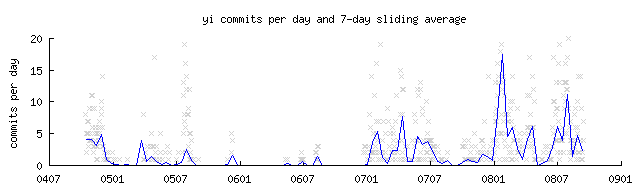
\includegraphics[width=\columnwidth]{activity}
}

\frame{
  \frametitle{Haskell support}
  Demo
}

\frame{
  \frametitle{Language support}
  \begin{itemize}
     \item Lexical analysis
     \item Syntax analysis (special parser combinators)
     \item AST-based highlighting
     \item AST available in mode-dependent functions
     \item Haskell: paren matching, layout, ...
  \end{itemize}
}

\frame{
  \frametitle{Configuration}
  Demo
}

\frame{
  \frametitle{Configuration}
  \itemize{
          \item Yi is a library (cf. XMonad)
          \item Users ``configure'' Yi by combining building blocks 
          \begin{itemize}
            \item no update of state (emacs)
          \end{itemize}
          \item Keymaps are (almost) parser combinators
          \begin{itemize}
            \item Parsing the input stream of event
            \item Produces a stream of actions
          \end{itemize}
          \item Type-system to control effects, guide user.
          \begin{itemize}
            \item IO
            \item Editor
            \item Buffer (DSL for buffer operations!)
            \item Pure functional
            \item Finger Tree of buckets
          \end{itemize}
        }
}


\frame{
  \frametitle{Conclusion}
  \begin{itemize}
    \item Usable
    \item Haskell support
    \item Try it!
    \item \texttt{http://haskell.org/haskellwiki/Yi}
    \item \texttt{cabal install yi -fvty}
    \itemize{
      \item create your \texttt{\$HOME/.yi/yi.hs}
      \item \texttt{http://code.haskell.org/yi/examples/yi.hs}
    }
  \end{itemize}
}

\frame[shrink=10]{
  \frametitle{Credits}
    \begin{tabular}{lll}
Allan Clark & Alson Kemp & Andres Loeh \\
Andrew Birkett & Andrii Zvorygin & Bastiaan Zapf \\
Ben Moseley & Cale Gibbard & Corey O'Connor \\
Daniel McAllansmith & Don Stewart & Duncan Coutts \\
Evan Martin & Fraser Wilson & Gustav Munkby \\
Gwern Branwen & Harald Korneliussen & Henning Guenther \\
Jason Dagit & Jean-Philippe Bernardy & Jeff Wheeler \\
Jens Petersen & Krasimir Angelov & Mario Lang \\
Mark Wotton & Massimiliano Gubinelli & Michael Maloney \\
Nicolas Pouillard & Paulo Tanimoto & Samuel Bronson \\
Scott Williams & Sean Leather & Shae Erisson \\
Simon Winwood & Spencer Janssen & Stefan O'Rear \\
Suleiman Souhlal & Taral & Thomas Schilling \\
Tim Newsham & Tristan Allwood & Tuomo Valkonen \\
Vivian McPhail & Yang Zhang
   \end{tabular}
}

\frame{\frametitle{Extra}}




\frame{
  \frametitle{Features}
      \begin{itemize}
        \item Usable editor
        \begin{itemize}
          \item Buffers, Copy/Paste, Search/Replace, Undo, ...
          \item Windows, Tabs, Syntax highlighting, ...
        \end{itemize}
        \item Keymaps: vim, emacs, (cua)
        \item Frontends: {\bf terminal}, gtk, cocoa
        \item Language support: Haskell, \LaTeX, perl, python, ...
        \item (Functional) Configuration in Haskell 
      \end{itemize}
}

\frame{
  \frametitle{Architecture overview}
  \begin{itemize}
    \item Written in Haskell!
    \item Keymap = Input $\leadsto$ [Action]
    \begin{itemize}
      \item parsers (combinators) of input
    \end{itemize}
    \item Action $\in$ stack of monads
    \begin{itemize}
       \item IO
       \item Editor
       \item Buffer (functional)
    \end{itemize}
    \item Abstracted UIs
    \item Language support
    \begin{itemize}
      \item Lexical analysis
      \item Syntax analysis (special parser combinators)
      \item AST-based highlighting
      \item AST available in mode-dependent functions
    \end{itemize}
    \item Uses about 30 packages 
  \end{itemize}
}


\frame{
  \frametitle{Haskell Support}
      \begin{itemize}
        \item Paren matching
        \begin{itemize}
          \item Layout aware
        \end{itemize}
        \item Auto indent
        \item Layout-preservation
        \item Ghci
        \item Cabal build
        \item (GHC API)
      \end{itemize}
}

\frame{
  \frametitle{Demo}
  \note{
       \begin{itemize}
        \item Haskell Support
        \item Latex
       \end{itemize}
  }
}


\end{document}